\documentclass[a4paper, 10pt]{article}
% Packages
\usepackage[utf8]{inputenc}  % For Unicode support
\usepackage{amsmath}         % For math symbols
\usepackage{graphicx}        % For including images
\usepackage{hyperref}        % For hyperlinks
\usepackage{graphicx}        % For image rendering
\usepackage{listings}        % For code blocks
\usepackage{sectsty}         % For section font formatting
\usepackage[a4paper, total={7in,9.5in}]{geometry} % For Margins
\usepackage{xcolor}
\usepackage{hyperref}
\usepackage{mathptmx}
\usepackage{tikz}
\usetikzlibrary{shapes.geometric}

% Package Initialization
\graphicspath{{images/}}

% Formatting
\sectionfont{\fontsize{16}{14}\selectfont}
\hypersetup{
    colorlinks=true,
    linkcolor=blue,
    filecolor=magenta,
    urlcolor=cyan,
}
% Define the style for C++ code
\lstdefinestyle{cpp}{
    language=C++,
    basicstyle=\ttfamily\small,
    keywordstyle=\color{blue},
    stringstyle=\color{red},
    commentstyle=\color{gray},
    morecomment=[l][\color{magenta}]{\#},
    % numbers=left,
    numberstyle=\tiny\color{gray},
    stepnumber=1,
    numbersep=8pt,
    showstringspaces=false,
    breaklines=true,
    % frame=single,
    rulecolor=\color{black},
    backgroundcolor=\color{white},
    tabsize=2,
    captionpos=b
}

% Define style for flowcharts
\tikzstyle{startstop} = [rectangle, rounded corners, minimum width=2cm, minimum height=1cm,text centered, draw=black, fill=red!30]
\tikzstyle{io} = [trapezium, trapezium left angle=70, trapezium right angle=110, minimum width=2cm, draw=black, fill=blue!30]
\tikzstyle{process} = [rectangle, minimum width=2cm, minimum height=1cm,text centered, draw=black, fill=orange!30]
\tikzstyle{decision} = [diamond, minimum width=2cm, minimum height=1cm,text centered, draw=black, fill=green!30]
\tikzstyle{arrow} = [thick,->,>=stealth]

% Title, author, date
\title{A Tour of C++}
\author{ksolomon}
\date{\today}

\begin{document}

\maketitle

\begin{abstract}
	Notes on Compilers Course
\end{abstract}


%%%%%%%%%%%%%%%%%%%%%%%%%%%%%%%%%%%%%%%%%%%%%%%%%%%%%%%%%%%%
% Chapter 1 - Introduction
%%%%%%%%%%%%%%%%%%%%%%%%%%%%%%%%%%%%%%%%%%%%%%%%%%%%%%%%%%%%

\section{Introduction}
\subsection{Introduction}
Compilers make generic executable which can run offline and process variable inputs to generate outputs. Interpreters run on data and translation unit in parallel to generate the output. Interpreters are much slower and any change to either data or program requires reinterpretation. As a result interpreters have lost favor. Fortran (Formula translation @ John Backus) was first major breakthrough in coding language (1950s) which inspired more research into computer science and became first compiler. Modern compilers still have similar data flow to Fortran.
\begin{figure}[ht]
	\centering
	\includegraphics[width=0.7\textwidth]{intro.compilerInterpreter.png}
	\caption{Compilers vs. Interpreters}
\end{figure}

\paragraph{Steps of the Compiler:}
\begin{enumerate}
	\item Lexical Analysis
	\item Parsing
	\item Semantic Analysis
	\item Optimization
	\item Code Generation
\end{enumerate}
\subsection{Structure of Compiler}
\begin{description}
	\item[Lexical Analysis:] is the process of breaking a program down into a series of tokens that are recognizable by the compiler.
	      definition
\end{description}
\begin{description}
	\item[Parsing:]
	      is the process of converting the tokens into an abstract syntax tree.
\end{description}
\begin{figure}[ht]
	\centering
	\includegraphics[width=0.4\textwidth]{intro.parsingEnglish.png}
	\includegraphics[width=0.4\textwidth]{intro.parsingCode.png}
	\caption{Example of parsing English vs Code}
\end{figure}
\begin{description}
	\item[Semantic Analysis:] is the process of checking the correctness of the program. In an ideal world this would fully understand the meaning of the program, however this is currently too hard for modern compilers. Ambiguity is a big issue in semantic analysis, so programming languages define strict syntactical rules to compile.
\end{description}
\begin{description}
	\item[Optimization:] is the process of reducing the size of the program to make it run faster, use less memory/power/networking/api calls, etc.
\end{description}
\begin{description}
	\item[Code Generation:] is the process of generating the actual machine code from the abstract syntax tree.
\end{description}
\begin{figure}[ht]
	\centering
	\includegraphics[width=0.7\textwidth]{intro.compilerRatio.png}
	\caption{Ratio of time spent in each step of compilers. In modern: small means well-understood/developed tools.}
\end{figure}
\subsection{Economy of Programming Languages}
\paragraph{Why so many languages?}
Application domains have different/conflicting needs. E.g. Scientific computing: good FP precision, array/matrix operations, parallelism. vs Business: persistence, reporting, data analysis.
\paragraph{Why new languages?}
Programmer training is the dominant cost for a programming language. Widely-used languages are slow to change. Cost to start a new language is low (since no responsibility to existing users). If productivity of new language is higher than maintenance of existing languages and training cost is low then they're incentivized to switch. New languages arise to meet gap in existing, more widely adopted, languages. New languages tend to look like old languages, since that can reduce the training cost (e.g. Java vs C++).
\paragraph{What makes a good language?}
There is no universally accepted metric to judge a language. Can't optimize what isn't defined.
\section{Cool}
\subsection{Overview}
\paragraph{COOL:}
Classroom Object-Oriented Language. Probably the only language with more compilers written than programs. Designed to be implemented quickly. Gives a taste of:
\begin{itemize}
	\item Abstraction
	\item Static Typing
	\item Inheritance
	\item Memory Management
\end{itemize}
Compile Cool into MIPS asm.

In 5 assignments:
\begin{enumerate}
	\item Write a Cool Program
	\item Lexical Analysis
	\item Parse
	\item Semantic Analysis
	\item Code generation
	\item Optional: Optimization
\end{enumerate}
\section{Lexical Analysis}
\subsection{Intro}
\paragraph{Goal}
\begin{itemize}
	\item Partition input string into lexemes
	\item Identify token of each lexeme
\end{itemize}
\paragraph{Token Class}
Correspond to sets of strings.
\begin{itemize}
	\item English: Noun, Verb, Adjective, etc.
	\item Programming Token Classes
	      \begin{itemize}
		      \item Identifiers: \texttt{abc123}
		      \item Integers: \texttt{123}
		      \item Keywords: \texttt{if, else}
		      \item Whitespace: \texttt{space, newline, tab, vertical tab, formfeed, etc.}
		      \item Punctuation:
		            \begin{itemize}
			            \item (
			            \item )
			            \item ;
			            \item =
		            \end{itemize}
		      \item Operator: \texttt{+ - * / ==}
	      \end{itemize}
\end{itemize}
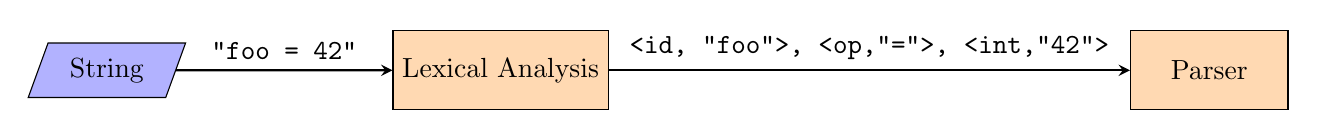
\begin{tikzpicture}
	\node (input) [io] at (0,0) {String};
	\node (la) [process] at (5,0) {Lexical Analysis};
	\draw [arrow] (input) -- (la) node[midway, above] {\verb!"foo = 42"!};
	\node (p) [process] at (14,0){Parser};
	\draw [arrow] (la) -- (p) node[midway, above] {\verb!<id, "foo">, <op,"=">, <int,"42">!};
\end{tikzpicture}
\newline Each identified token is a "lexeme".
\subsection{Examples}
\paragraph{Fortran}
Whitespace is ignored. So \verb!VAR1! is the same thing as \verb!VA    R1!. This rule was implemented because in punchcard days it was very easy to accidentally add whitespace.
Only way to distinguish between below two examples is to implement "lookahead" for punctuation. Lookahead creates complication in compiler logic. It is always needed, but it is a good idea to define upper bounds on complexity.
\begin{lstlisting}[style=cpp]
DO 5 I = 1,25 // do-loop where loop extends from DO down to statement 5
DO 5 I = 1.25 // assignment of DO5I=1.25
\end{lstlisting}
\paragraph{PL/1}
Keywords are not reserved. Example legal code:
\verb!IF ELSE THEN THEN = ELSE; ELSE ELSE = THEN!
This made lexical analysis much harder.
\begin{lstlisting}[style=cpp]
DECLARE (ARG1, ..., ARGN) // DECLARE can be keyword or array reference in given context. This requires unbounded lookahead since you'd have to scan ahead of ARGN in order to actually know
\end{lstlisting}
\paragraph{C++}
\begin{lstlisting}[style=cpp]
Foo<Bar>; // Template Syntax
cin >> var; // Stream Syntax
\end{lstlisting}
This creates a conflict with nested templates (\verb!Foo<Bar<Buzz>>!) and older compliers would often require extra whitespace between last two \verb!> >! in order to not treat as syntax error.
\subsection{Regular Languages}
Regular Languages (syntax) specify regular languages (set of legal strings).
\paragraph{Regular Expression Constructs}
\begin{itemize}
	\item single character: (A)
	\item $\epsilon$: (the empty string "")
	\item union: (A+B)
	\item concatenation: (AB)
	\item iteration: (A*) where $(A^0 = \epsilon)$
\end{itemize}
\paragraph{Given a language $(\Sigma) = {0,1}$} this can be represented as the following sets of strings:
\begin{itemize}
	\item $1^* = \bigcup_{i>=0}1^i$ = {1, 11, 111, ...}
	\item $(1+0)1$ = $\{ab | a \in 1+0  \land b \in 1\} = \{11,01\}$
	\item $0^*+1^*$ = $\{0^i | i >= 0\} \cup \{1^i | i >= 0\}$
	\item $(0+1)^*$ = $ \bigcup_{i>=0}(0+1)^i $ = $\Sigma^*$ (all strings of 0's and 1's aka the superset of the language)
\end{itemize}
\subsection{Formal Languages}
Play a large role in theoretical computer science.
\begin{description}
	\item[Formal Language] Let $\Sigma$ be a set of characters (alphabet). Then the language $L$ is a formal language over $\Sigma$ if it is a subset of $\Sigma*$.
\end{description}
\begin{itemize}
	\item Alphabet = English characters, Language = English sentences (not exactly formal since not all sentences are agreed upon).
	\item Alphabet = ASCII, Language = C programs (this IS a formal language).
\end{itemize}
\begin{description}
	\item[Meaning Function] Let $L$ be a formal language. Then the meaning function $M : L \rightarrow \Sigma^*$ is a function that maps each string in $L$ to a string in $\Sigma^*$. Aka maps syntax to semantics (meaning).
\end{description}
\section{Lexical Specifications}
\begin{figure}[ht]
	\centering
	\includegraphics[width=0.7\textwidth]{intro.formalLanguages.png}
	\caption{L (Meaning Function) is a map from Expressions to Sets of Strings}
\end{figure}
Purpose of using a Meaning function is to:
\begin{itemize}
	\item Decouple Syntax from Semantics
	\item change syntax without changing semantics (optimize)
	\item Expressions do not have a 1:1 relationship with meanings. Generally N:1 (multiple ways to say/write the same thing)
\end{itemize}
\paragraph{Regular Expressions}
\begin{itemize}
	\item Keyword: "if" or "else" or "then" or ... $'if' + 'else' + 'then'$
	\item Integer: non-empty string of digits: $'0' + '1' + '2' + '3' + '4' + '5' + '6' + '7' + '8' + '9'$, however can't be empty string so instead of digit $digit^*$ we can write this as $digit^+$
	\item Identifier: strings of letters or digits starting with a letter, where letter = [a-zA-Z]. $letter(letter + digit)^*$
	\item Whitespace: non-empty sequence of $(blanks/newlines/tabs)^+$
\end{itemize}
anyone1@cs.stanford.edu: $letter(letter + digit)^* + @ + letter^+ + . + letter^+ + . + letter^+$
\paragraph{PASCAL}
\begin{itemize}
	\item digits = $digit^+$
	\item optFraction = $('.'digits) + \epsilon $ where $\epsilon$ means empty set is valid
	      \begin{itemize}
		      \item ('.'digits)?
	      \end{itemize}
	\item optExponent = $('E' ('+' + '-' + \epsilon) digits) + \epsilon$
	      \begin{itemize}
		      \item ('E'('+'+'-')?digits)?
	      \end{itemize}
	\item number = $digits + optFraction + optExponent$
\end{itemize}
Question mark (?) means the aforementioned component is optional
\begin{figure}[ht]
	\centering
	\includegraphics[width=0.5\textwidth]{lexicalSpec.png}
	\caption{Regular Expression Notation}
\end{figure}
\paragraph{Given string s and regular expression r, is it in the language (L) of a regular expression?}
$s \in \mathcal{L}(r)$?
\paragraph{Lexical Specification:}
\begin{enumerate}
	\item Write a rexp for the lexemes of each token class
	      \begin{itemize}
		      \item Number: $digit^+$
		      \item Keyword: $if | else | ...$
		      \item Identifier: $letter(letter + digit)^*$
		      \item OpenPar: $($
		      \item ...
	      \end{itemize}
	\item Construct R, matching all lexemes for all tokens i.e $R = Keyword + Identifier + Number + OpenPar + ...$
	\item Let input be $x_1 ... x_n$. For $1 <= i <= n$ find $x_1 ... x_n \in \mathcal{L}(R)$?
	\item If success, then we know that $x_1 ... x_n \in \mathcal{L}(R_j)$ for some $j$
	\item Remove $x_1 ... x_i$ from input and jump to step 3
\end{enumerate}

\begin{description}
	\item[Maximal Munch:] when faced with a choice of two different prefixes for input of different length, always take the longer one
\end{description}

\begin{description}
	\item[Ambiguous Class?]
	      When there are multiple possible classes for a given token, use priority queue to determine which one to use.
\end{description}

\begin{description}
	\item[No Rule Matches?]
	      Match error (as base case when other things don't match) " all strings not in the lexicon"
\end{description}

\begin{description}
	\item[What makes a good algorithm?] Requires only single pass over input, Few operations per character (table lookup)
\end{description}
\subsection{Finite Automata}
A good implementation model for regular expressions where regular expressions are the specification and finite automata are the implementation.
\begin{description}
	\item[Finite Automata:]
	      \begin{itemize}
		      \item input alphabet $\Sigma$
		      \item set of states $S$
		      \item state start state $n$
		      \item set of accepting states $F \subseteq S$
		      \item set of transitions $state \rightarrow^{input} state$
	      \end{itemize}
\end{description}
\subsection{RegEx to NFAs}
\subsection{NFA to DFA}
\subsection{Implementing Finite Automata}
\section{Assignment 1}

\end{document}
